%!TEX root = ../dissertation.tex
%--------------------------------------------------
% \begin{savequote}[75mm]
% \qauthor{Quoteauthor Lastname}
% \end{savequote}
%-------------------------------------------------- 

\chapter{Dynamics of genome size evolution in insects}
\label{cha:dynamics}

\section{Introduction}

Genome size variation is an important aspect of eukaryote genome
evolution \citep{Gregory2005,Petrov2001} and seems positively correlated
with cell size \citep{Dufresne2011}, and body size in invertebrates
\citep{Gregory2008}. Genome size has also been linked to cell division
time \citep{Bennett1977} and developmental rate \citep{White2000}.
Genome size variation does not appear to be correlated with organismic
complexity \citep{Gregory2007}. Therefore, understanding modes and
processes of DNA gain and loss is a necessary prerequisite to understand
the relationship between genome size and phenotypic traits.

Studies on genome size evolution have been published dealing with taxa
with either high variation in genome sizes, such as flowering plants
\citep{Bennetzen2005,Piegu2006,Vitte2007,Kelly2015}, conifers
\citep{Nystedt2013} \cite{Nystedt2013}, and teleost fish
\citep{Blass2012}, or dealing with species with extreme genome sizes,
such as pufferfish \citep{Neafsey2003} with an extremely small genome or
salamanders \citep{Sun2012} with extraordinary large genomes. Especially
in teleost fish, cases of whole genome duplication play a major role in
genome size variation \citep{Sato2010,Marburger2018}. Mammals and birds,
which display relatively low variation in genome size, have been subject
to research as well \citep{Kapusta2017a}.

At least in teleost fish, genome size variation is correlated with
genome duplications. In many other instances, the frequency of
transposable elements (TEs) in genomes has been found to be correlated
with genome expansion and contraction \citep{Sotero-Caio2017}. In insects
and crustaceans, genome size dynamics are correlated with TE content but
also show a phylogenetic pattern \citep{Alfsnes2017,Petrov1996,Petrov2000}. TEs appear to play
a pivotal role in insect genome size evolution that is not fully
explained by variation of TE content (reviewed in \citet{Maumus2015}).

In insects, there is no reason not to expect TE activity and DNA
gain/loss rate to be phylogeny dependent, similar to what has been
documented in mammals and birds \citep{Kapusta2017a}. Analogously, there
would also be phylogenetic signal in TE content and TE copy divergence
(age). In mammals and birds, an ``accordion'' model of genome size
dynamics has been proposed \citep{Kapusta2017a} that predicts a more or
less stable genome size over time. According to this model, genome
expansion due to TE activity is counteracted by DNA removal, allowing
little fluctuations in genome size. In insects, however, where most
insect orders are much older than the mammal and bird lineages, and in
the face of burst-like transposition events, it may be impossible to
observe an ``accordion'' model of genome size dynamics on a pan-ordinal
scale in insects. In the present study, we exploit the growing number of
sequenced insect genomes and conduct an integrated analysis to assess
genomic DNA gain and loss caused by TE activity. Our results are
inconsistent with an ``accordion'' model of genome size dynamics,
therefore we propose that genome size in insects is governed by
different dynamics than in mammals and birds.

\section{Methods}

\subsection{Ancestral genome size
estimation}

To determine the age of TE copies in the insect genomes, we first
estimated clade-specific ancestral genome sizes with the approach
described in the following. We sourced the Animal Genome Size Database
\citep{Gregory2018} (\url{http://genomesize.com}, accessed 2018-05-01) to
obtain genome size estimates for 1,514 arthropod species. Additionally,
we exploited the BOLD database \citep{Ratnasingham2007}
(\url{http://www.boldsystems.org}, accessed 2018-03-19) to obtain
1,571,820 COI barcode nucleotide sequences for 105,397 arthropod
species. Of these, we identified 605 species that were represented in
both databases. We included our own genome size estimates for eight
additional species (supplemental Table S4), bringing the total number of
species to 613.

For the proturan \emph{Catajapyx aquilonaris}, we added COI data by
retrieving a COI sequence from the closely related species
\emph{Gollumjapyx smeagol} (GenBank ID DQ993154.1) and using it as query
in a BLAST search in the genome assembly provided by the i5k initiative
(source see supplementary Table S1). We received two hits and used the
longer one (scaffold131247\_cov1551 positions 852-1522) as query in a
BLAST search in GenBank. The reciprocal search hit the mitochondrial
genome of \emph{Japyx solifugus} (Accession AY771989.1), another closely
related species, which confirmed that our hit was indeed the COI
sequence of \emph{C. aquilonaris}.

To obtain a phylogenetic tree with branch length estimates, we first
compiled the constraint tree topology from the literature. The arthropod
order topology was taken from \citep{Misof2014}. We computed multiple
sequence alignments from the COI sequences for each order separately
using MAFFT v7.309. We removed redundant sequences and sequences that
could not be translated without having stop codons. and inferred ML
phylogenies for each order using RAxML v8.2.11. We corrected these
order-specific topologies using published phylogenies (reference list in
supplemental Table S2). For those species without placement from the
literature, we used the COI topology under majority-rule consensus in
case there were more than one COI sequence. Then we used that topology
as constraint in a branch length estimate using RAxML:

\begin{verbatim}
raxml -s COI_nt_seq.afa -n COI -m GTRCAT -p 1 -g CONSTRAINT.tree
\end{verbatim}

The resulting tree was rendered ultrametric by a short Python script
using the ETE toolkit \citep{Huerta-Cepas2016}. To time-calibrate the
phylogeny, we selected calibration points from \citep{Misof2014} (Table
S4) and used the \texttt{chronos} function from the ape package in R to
adjust the branch lengths. We used the upper and lower bounds of the 95
\% confidence interval as minimum and maximum node ages. We set
$\lambda$ to 2 and used the discrete model. We used the
\texttt{fastAnc} ML implementation in the phytools package
\citep{Revell2012} in R to infer ancestral genome sizes using the
Ornstein-Uhlenbeck model for each node along the tree including 95 \%
confidence intervals.

\subsection{Genomic datasets}

The genome assembly versions and data sources of 96 arthropod species
are listed in supplemental Table S1. The genome assemblies were
downloaded from NCBI (TODO X species) or from the i5k FTP server (TODO Y
species). Genome size estimates were obtained from the Animal Genome
Size Database (\citep{Gregory2018}, \url{http://genomesize.com}),
measured in our own lab using flow cytometry (FCM), or estimated using a
\emph{k}-mer peak method adopted from \citet{Hozza2015}. Our own
estimate results are listed in supplemental Table S4).

\subsection{Transposable element
annotation}

We used a custom pipeline for repeat annotation that employs
RepeatModeler 1.0.10 \citep{Smit2015} to infer a species-specific
repeat consensus library from each genome assembly, and RepeatMasker
4.0.5 \citep{Smit2015a} to annotate TE copies in the genome
assemblies. The annotation by RepeatModeler includes a substantial
fraction of ``Unknown'' elements, so we added an intermediate filtering
step to exclude false positives. We used NCBI BLAST to search the
consensus libraries in the NCBI non-redundant nucleotide database, and
removed all ``Unknown'' consensus sequences that did not result in a hit
on a known TE protein. We also removed annotations shorter than 50
nucleotides.

To infer accurate TE content estimates and TE ages from the RepeatMasker
annotation results, we developed a Perl program that uses the Kimura
distance of each TE copy from the TE consensus sequence and the
order-specific nucleotide substitution rate to infer the age of each TE
copy in million years (My). We used a time-calibrated phylogeny of
insects \citep{Misof2014} and multiple sequence alignments of 1,478
protein-coding genes from 144 arthropod species \citep{Misof2014} to
infer order-specific nucleotide substitution rates by using the weighted
arithmetic mean of substitution rates (see equation (S1) in supplemental
material). The program also takes into account that TE annotations
sometimes overlap each other by distributing the count of affected
nucleotide positions as fractions evenly among overlapping TE copies.
While this approach results in decimal instead of integer TE lengths, it
provides a better estimate of the amount of nucleotides covered by TEs
as it handles each element equally. The corrected lengths were only used
in the TE content counts, not in the age estimations.

\subsection{DNA gain and loss}

We classified TEs into clade-specific and ancient based on the age
estimates (a TE copy was ancient if it was older than the clade it was
found in), and calculated the amount of DNA gained as the amount of
clade-specific TEs. For Chelicerata and Myriapoda, we took clade
divergence times from \citet{Misof2014} (all divergence times are
listed in Table S1).

With the ancestral genome sizes and the inferred amounts of DNA gained
by TE activity, we computed the amount of ancestral DNA in the extant
genomes by subtracting the amounts of lineage-specific TE material from
the extant genome assembly sizes. This allowed us to infer the amount of
ancestral DNA that was lost since the common ancestor of the clade for
each arthropod lineage by subtracting the amount of ancestral DNA from
the estimated ancestral genome size.

We computed the DNA loss coefficient $k$ according to
\citet{Lindblad-Toh2005} as $E = A e^{-kt}$, where $E$ is
the amount of extant ancestral sequence in the genome assembly,
$A$ the total ancestral assembly size, and
$t$ the time since the split from the last ancestor.

\begin{equation}
k = \ln{\frac{A}{E}}
\end{equation}

\section{Results}

\subsection{Ancestral genome size
reconstruction}

We reconstructed ancestral genome sizes using a concatenated phylogeny
of 613 arthropod species based on published phylogenetic relationships
(refs. listed in Supplemental Table S6) and genome size estimates for
the tip species from the genome size database \citep{Gregory2018}. We
used COI barcode sequences obtained from the BOLD database
\citep{Ratnasingham2007} to estimate the branch lengths. We inferred an
ancestral genome size for hexapods between 782 and 1943 Mbp (95 \%
confidence interval) (Figure \ref{fig:ancestral-sizes} on page
\pageref{fig:ancestral-sizes}). This inferred genome size is well above
the maximum of many holometabolous clades such as Diptera (272 to 545
Mbp), Lepidoptera (318 to 738 Mbp), or Hymenoptera (303 to 633 Mbp)
(Table 1). Among the hemimetabolan orders, most inferred genome sizes
are within the range of the inferred ancestral genome size of hexapods,
except for Orthoptera, of which the ancestral size was inferred to be
between 3,677 and 9,473 Mbp. Indeed, the estimated genome sizes of
extant representatives of Orthoptera are between 2 Gbp in \emph{Acheta
domesticus} and 16.5 Gbp in \emph{Podisma pedestris}.

In some orders, we infer a dynamic pattern of genome size evolution. For
example within Lepidoptera, Papilionidae have smaller genome sizes than
every other Lepidopteran family, or the two sister groups Drepanidae and
Geometridae differ in their inferred ancestral genome size more than
twofold. (\emph{Drepana} species (Drepanidae), median size: 318 Mbp;
\emph{Scopula limboundata} (Geometridae), median size: 870 Mbp), as is
also the case for the two sister groups Notodontidae (\emph{e.g.},
\emph{Nadata gibbosa}; median size: 352 Mbp) and Erebidae (\emph{e.g.},
\emph{Malacosoma disstria}; median size: 636 Mbp). A similar pattern is
visible in Coleoptera: Tenebrionidae (such as \emph{Tribolium} species)
have small genomes (median size: 235 Mbp) in contrast to the
Cleridae/Silvanidae/Chrysomelidae/Curculionidae complex with large
genomes (\emph{e.g.}, \emph{Callosobruchus}; median: 836 Mbp), and
within Carabidae, the \emph{Carabus} lineage (245 Mbp) stands in stark
contrast to the other carabid species \emph{Calosoma scrutator} (1,017
Mbp).

\begin{figure}[h!]
\begin{center}
\includegraphics[width=\textwidth]{COI-tree-with-genome-sizes-log}
\caption[Ancestral genome size reconstruction reveals highly dynamic insect
genomes]{{Ancestral genome size reconstruction reveals highly dynamic insect
genomes.
{\label{fig:ancestral-sizes}}%
}}
\end{center}
\end{figure}

The smallest extant and ancestral inferred genome size was found in
Strepsiptera (MRCA: 104 to 349 Mbp, with the extant \emph{Xenos
vesparum} having 127 Mbp). The ancestral holometabolan genome was
inferred to be between 390 and 751 Mbp in size. Holometabola, however,
appear to have undergone several events of genome size contraction
according to our inferences. For example, the MRCA of basal Hymenoptera
such as \emph{Macrocentrus cingulum}, \emph{Aphidius colemani}, and
\emph{A. ervi} has an inferred ancestral genome size between 140 and 420
Mbp; similarly, we inferred a genome size of 199 to 464 Mbp for the MRCA
of the \emph{Tribolium} beetle genus. Likewise, we inferred smaller
genomes for the MRCA of the nematocerans \emph{Telmatogeton japonicus}
and \emph{Chironomus plumosus} (Diptera, 166 to 354 Mbp) and of the
\emph{Drosophila} group (202 to 359 Mbp). Our inferences also include
examples of genome expansion. For example, the MRCA of dermestid beetles
had an inferred genome of between 560 and 1,459 Mbp); the MRCA genome of
\emph{Caenurgina crassiuscula} and \emph{Lymantria dispar} (Lepidoptera)
was inferred to be between 520 and 1,060 Mbp, and the MRCA genome of the
\emph{Aedes} mosquito genus was inferred to be between 591 and 1,224
Mbp. These results contradict prior suggestions that Holometabola
generally have smaller genomes than Hemimetabola, \emph{e.g.},
\citep{Hanrahan2011}.

\subsection{Transposable elements contribute to genome size
variation}

To further illuminate the evolutionary dynamics of genome size in
arthropods, we investigated the correlation between genome size and TE
content. We identified TEs in 96 arthropod genomes using an annotation
pipeline that combines RepeatModeler \citep{Smit2015} and RepeatMasker
\citep{Smit2015a}. We inferred the TE age distribution of the major TE
orders that include LINE, SINE, DNA, and LTR. Genome size correlates
with TE content (PIC \citep{Felsenstein1985}, Pearson's product moment
correlation, $p = 0.0003484$). The median ages of all TE classes
within species are significantly correlated with the divergence times of
the respective species order (Figure \ref{fig:median-ages} on page
\pageref{fig:median-ages}), but only LINEs show this
correlation also when applying PIC (Kendall's rank correlation,
$p = 0.04$).

Using divergence times from the dated phylogeny based on the literature
(see above), we classified the TE content into lineage-specific (younger
than the age of the lineage, \emph{i.e.}, the split of the species with
its last common ancestor) and ancient (older than the lineage). In 36
out of 53 insect species that occurred in the dated tree, we found more
than 99 \% lineage-specific TEs (Figure \ref{fig:ancient-vs-clade-age} on page
\pageref{fig:ancient-vs-clade-age}, Supplemental Figure S1\todo{add}).
Notable exceptions included the termite \emph{Zootermopsis} with 86.3 \%
ancestral TEs, the bumblebee \emph{Bombus terrestris} with 81.1 \%
ancestral TEs and the dragonfly \emph{Calopteryx splendens} with 82 \%
ancestral TEs. The closely related \emph{Drosophila} species displayed
great variation in the ancestral TE fraction, ranging from 0.85 \% in
\emph{D. mojavensis} to 47.4 \% in \emph{D. simulans}. We tested for
phylogenetic signal using Blomberg's \emph{K} and found low signal in
the ancestral TE fraction ($K = 0.1$, $p = 0.9$). The
fraction of ancestral TEs is significantly correlated with the species'
age under phylogenetically independent contrasts (PIC) (Kendall's
$\tau$, $p = 2e-10$.

\begin{figure}[h!]
\begin{center}
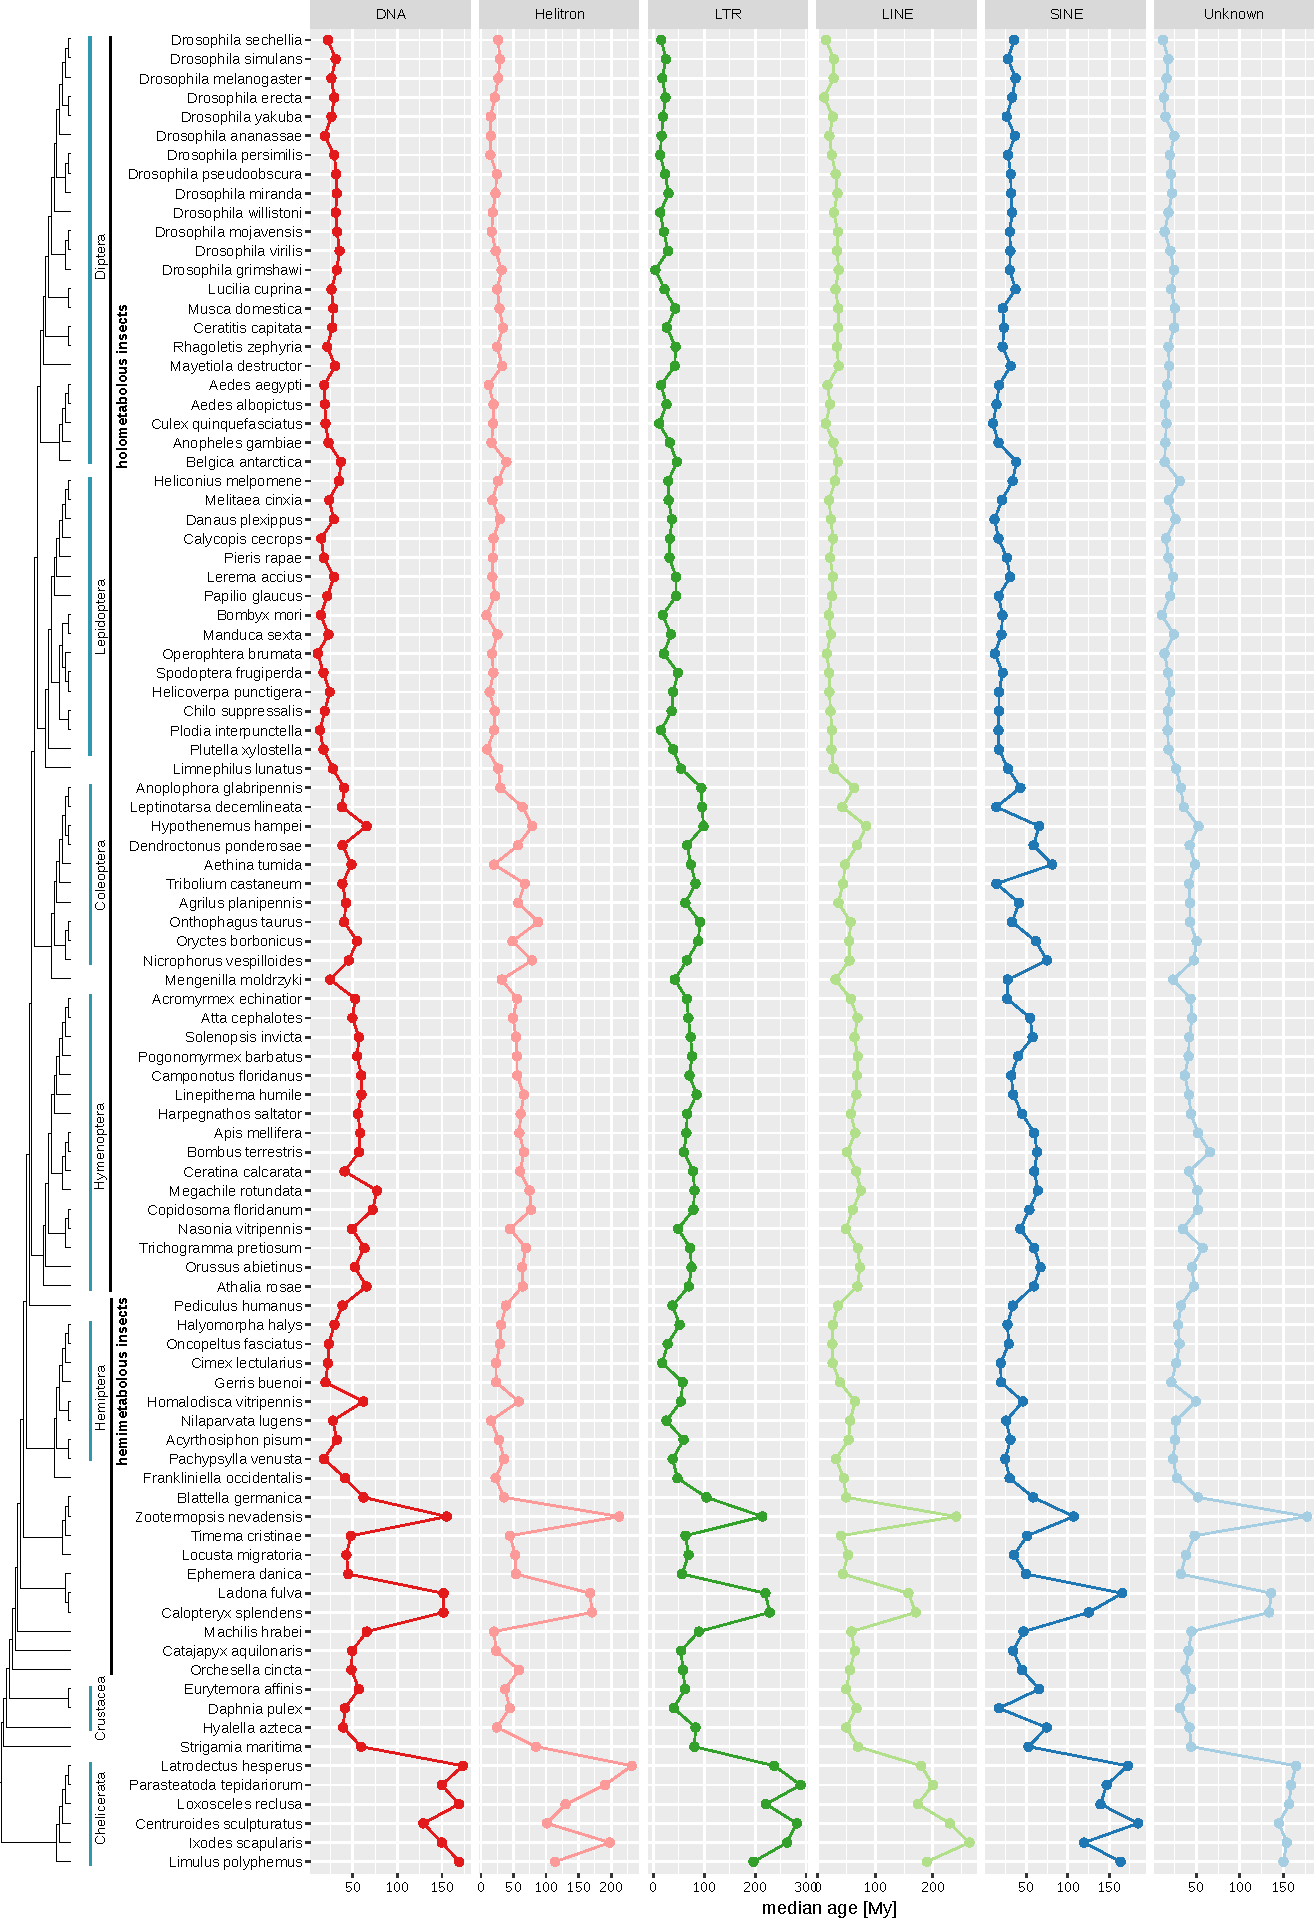
\includegraphics[height=0.9\textheight]{age-mediane}
\caption[Median ages of TE subclasses in arthropod genomes]{{The median ages of six TE subclasses in all sampled species show
variation between and within subclasses. Clade relationships after
\textbackslash{}citet\{Misof2014\}. Species relationships within clades
are based on the published phylogenies listed in the supplement.
{\label{fig:median-ages}}%
}}
\end{center}
\end{figure}

\begin{figure}[h!]
\begin{center}
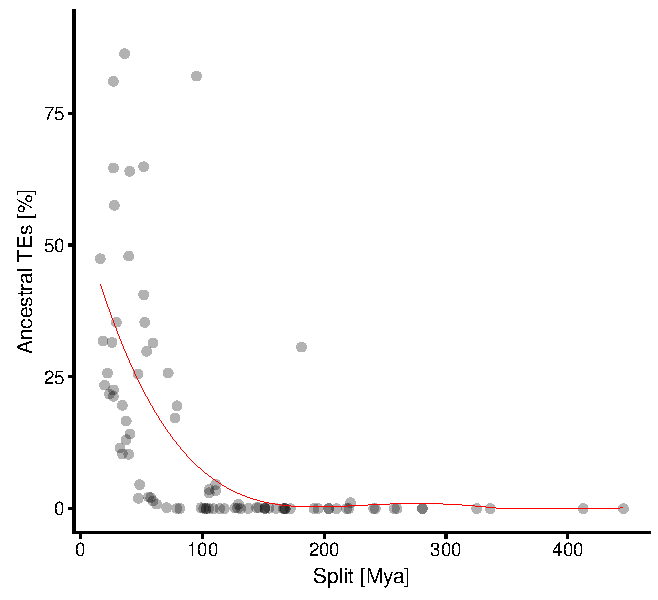
\includegraphics[width=0.70\textwidth]{age-vs-perc-ancestral}
\caption[TEs are no longer recognized as ``ancient'' beyond a clade age of
\textasciitilde{} 120 Mya]{{TEs are no longer recognized as ``ancient'' beyond a clade age of
\textasciitilde{} 120 Mya. Dots: individual measurements; red line:
polynomial regression.
{\label{fig:ancient-vs-clade-age}}%
}}
\end{center}
\end{figure}

We inferred the total amount of DNA gained and lost in each lineage by
first calculating the fraction of ancestral DNA: we subtracted the
amount of lineage-specific TEs (DNA gained since the split of the
sister-species present in our tree) from the assembly size of each
species (Fig. \ref{fig:gain-loss} on page \pageref{fig:gain-loss}. To compute the amount of DNA lost, we subtracted the amount of
ancestral DNA from the inferred ancestral genome size of each species.
This analysis revealed highly dynamic genome sizes among species and
clades (Figure \ref{fig:ancient-vs-clade-age} on page
\pageref{fig:ancient-vs-clade-age},
Table S2\todo{TABLE?}). In 75 out of 89 species (we omitted the
chelicerates and myriapods which were not represented in the dated
phylogeny), the amount of DNA loss exceeds the amount of DNA gained
through the accumulation of TEs. These 75 species include five
dipterans, in particular two representatives of \emph{Aedes} mosquitoes,
but no representatives of \emph{Drosophila} or other closely related
species. The ratio of gain to loss ranged between 0.2 in the fly
\emph{Rhagoletis zephyria} to 5.1 in the butterfly \emph{Calycopis
cecrops}.

\begin{figure}[h!]
\begin{center}
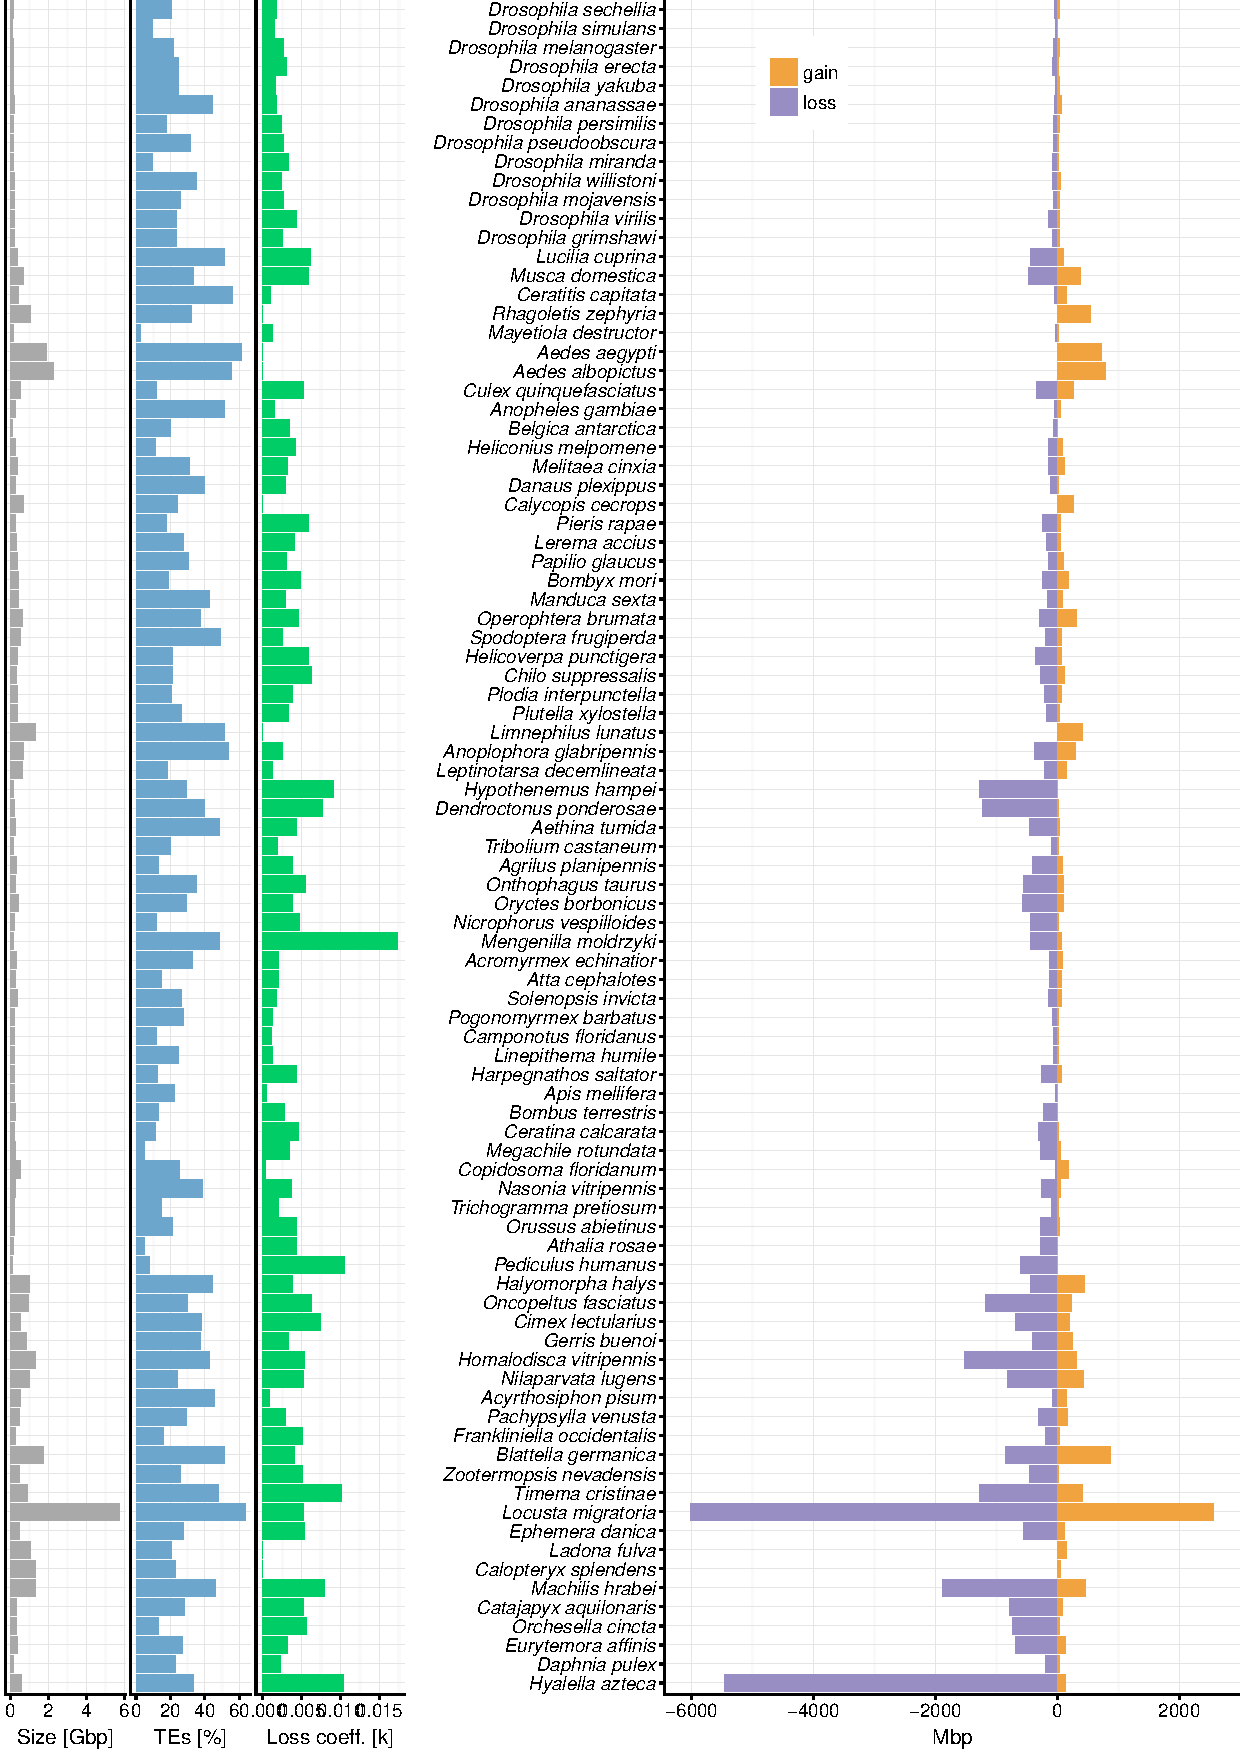
\includegraphics[height=0.93\textheight]{gain-loss}
\caption[DNA gain and loss due to TE activity]{{Increased DNA loss rate explains some of the observed genome size
reductions in insects, but not all.
{\label{fig:gain-loss}}%
}}
\end{center}
\end{figure}

We inferred the largest absolute values of DNA gain (3.7 Gbp) and loss
(7.1 Gbp) in the largest studied genome, that of the locust
\emph{Locusta migratoria} with 5.8 Gbp. It is followed by the amphipod
\emph{Hyalella azteca}, which was inferred to have lost 5.4 Gbp, but
gained only 136 Mbp. Crustaceans in general appear to have lost large
absolute amounts of DNA, however the average ratio of DNA gain to DNA
loss (0.11) is estimated to be lower than that in hexapods (0.88). The
ratio of DNA gain to DNA loss was not significantly different in
holometabolous insects from that in hemimetabolous insects (ANOVA,
$p = 0.5$).

From the DNA gain and loss analysis, we calculated DNA loss coefficients
according to \citep{Kapusta2017a} (see Methods). The less coefficient,
$k$, expresses the rate of DNA loss as a function of
time, taking into account the ancestral genome size and the amount of
ancestral DNA in the extant genome. We found an extremely high DNA loss
coefficient in the strepsipteran \emph{Mengenilla moldrzyki} with a
small genome (156 Mbp, 48.5 \% TEs; $k = 0.0173$). We found the
lowest DNA loss coefficients in the two mosquitoes \emph{A. aegypti}
(1,871 Mbp, 61.2 \% TEs, $k \approx 0$) and \emph{A. albopictus}
(2,247 Mbp, 55.6 \% TEs, $k \approx 0$), both of which have large
genomes and a high TE content. Interestingly, assembly size and DNA loss
coefficient are negatively correlated (Kendall, PIC, $p = 0.001$)
in contrast to a weak positive correlation between TE content and DNA
loss coefficient (Pearson, PIC, $p = 0.03$). Without PIC, there
is no correlation at all (Supplemental Figure S2 \todo{add these
figures}).



\section{Discussion}\label{discussion}

In this study, we present the most comprehensive systematic analysis of
genome size dynamics during arthropod evolution with a focus on gain and
loss of TE-derived DNA to date. In arthropods, and particularly in
hexapods, genome sizes are not nearly as stable as they are among
mammals and birds \citep{Kapusta2017a}, but instead show large variation
up to 1,600 \% (Figure \ref{fig:ancestral-sizes} on page \pageref{fig:ancestral-sizes}). For eutheria and aves, an ``accordion'' model
of genome size dynamics was proposed \citep{Kapusta2017a}, which predicts
that DNA loss counteracts DNA gain caused by lineage-specific TE
transposition, thereby maintaining a genome size equilibrium.
Mechanistically, the ``accordion'' model proposes that TE insertions
lead to DNA gain, but also generate targets for ectopic recombination
which can induce DNA loss. \citet{Kapusta2017a} further show that there is
empirical evidence in mammalian and bird genomes of frequent
macrodeletions compatible with the action of ectopic recombination.
Given the proposed mechanistic explanation of the ``accordion'' model,
it should also apply to arthropod genomes. In fact, we inferred a
similar balance of DNA loss and gain within the major insect orders
(large genome sizes are correlated with high TE content (Figure
S3\todo{add figure}) and
high amounts of DNA loss (Figure S2\todo{add figure})), but the ``accordion'' model does
not explain the large periodic shifts in genome size among the major
insect orders. Instead, insect genomes appear to cope with TE influx in
an entirely different manner than vertebrate genomes: Where in mammals,
a high rate of DNA loss leads to a smaller extant genome size, in
insects the genome size remains more or less constant according to our
DNA loss coefficient inferences (Figure S2\todo{add figure}). These results suggest that
in insect genomes, even a high rate of DNA loss is barely able to cope
with the high rate of DNA influx due to TE activity and keep the genome
size stable -- there is no apparent trend towards genome shrinkage in
insects.

Genome size reduction in vertebrates has been implicated in the
metabolic requirements of powered flight \citep{Wright2014}; this is
indicated by the fact that birds with higher metabolic rates, such as
hummingbirds, have smaller genomes than flightless birds
\citep{Gregory2005}. In insects, we would expect a similar rate of DNA
removal over time if powered flight should play a role. However, we
observe a different situation: in flightless arthropods, genome size
shows a trend to increase with the DNA loss coefficient, while in
insects capable of flight, the trend is downwards (Fig. S4\todo{add
figure}). Hence, the
metabolic rate is likely not a predictor of genome size in insects,
regardless of flight capability.

\subsection{Ancient TEs become
unrecognizable}\label{ancient-tes-become-unrecognizable}

We found almost no ancestral TEs in species that diverged earlier than
100 Mya from their sister species (Figure \ref{fig:ancient-vs-clade-age} on page
\pageref{fig:ancient-vs-clade-age}). This is most likely a
consequence of the TE nucleotide sequence similarity decaying over time
and thus sequence homology becoming undetectable. Its effect is easily
visualized when plotting the TE content distribution over the sequence
divergence (or age, if conversion is available) and dividing the
landscape in two parts, separated at the age of the species
(Supplemental Figure S3\todo{add figure}). These findings are in line with other studies
suggesting that inactive TEs become unrecognizable beyond 50 Mya due to
high sequence divergence (\emph{e.g.}, SINES \citep{Shedlock2000}).

\subsection{Limitations of the methods in insect
genomes}\label{limitations-of-the-methods-in-insect-genomes}

This analysis is of course heavily influenced by the node dating of the
underlying phylogeny, and our approach using COI barcode sequences
cannot rival the accuracy of phylogenomic studies (\emph{e.g.},
\citep{Misof2014}). However, using calibration points from
\citep{Misof2014} enabled us to estimate node ages with reasonable
accuracy and therefore provide a robust dated phylogeny for the TE age
classification. Unfortunately, for some species there were no closely
related species in the dataset, which forced us to select an ancestral
split that is older than the species would be. This was the case for all
orders with only a single representative (Collembola, Diplura, Psocodea,
Trichoptera, and Mecoptera). Here, the representative species were
assigned an age that is even older than the age of the sister order,
which likely lead to an underestimation of the ancestral TE content. To
solve this issue, genome size estimates for more representatives of
these orders are required. This also highlights the importance of
efforts like the genome size database \citep{Gregory2018} in the age of
whole-genome sequencing -- not only because the estimates aid in
establishing sequencing strategies, but also for comparative analyses
like this one.

\citet{Kapusta2017a} obtained a denser dataset that included a
multiple whole genome alignment of 100 vertebrate species. Using this
whole genome alignment, they were able to infer micro- and
macrodeletions in the vertebrate lineage. These are lacking in our
dataset simply because whole genome alignments are difficult in insects
due to low conservation of synteny: while the human genome aligns with
over 98 \% to the chimpanzee genome and with around 70 \% to the mouse
genome \cite{Mural2002} this is not the case in insects. For example,
the honey bee \emph{A. mellifera} genome aligns to less than 20 \% of
the turnip sawfly \emph{Athalia rosae} genome, also a representative of
the order Hymenoptera (A. Donath, \emph{pers. comm}). Thus, we omitted
analysis of micro- and macrodeletions and segmental duplications in the
insect genomes. However, since these events make up at most 10 \% of the
vertebrate DNA gain or loss \citep{Kapusta2017a}, with the analysis on
TEs we have covered the major source of DNA gain and loss in arthropod
genomes. Our analysis is instead based on a wider dataset with twice as
many species from all major insect and crustacean orders. This provided
us with a broad comparative view on genome size dynamics in arthropods.

\subsection{Genome contraction covaries with TE
expansion}\label{genome-contraction-covaries-with-te-expansion}

Insects have much larger effective population sizes than mammals or
birds, which limits the effects of genetic drift and exacerbates the
efficiency of natural and purifying selection \citep{Szitenberg2016}. As a
result, we would expect TE activity to both be of limited detrimental
effect to the host organism, and lead to widely distributed copies of
active TEs among the individuals of a population. The latter can happen
within a few generations, as has been shown in \emph{Drosophila} fruit
flies (TODO citation); our analysis suggest a similar rate of
intra-population TE proliferation in other insect species, however this
remains to be tested experimentally. The greatly increased reproductive
cycles in insects also add to \ldots{} {[}TODO\}

TE activity has been shown to be a pivotal agent shaping genome size
evolution in insects \citep{Maumus2015}, with DNA loss barely
counteracting DNA gained by TE transposition to maintain a genome size
equilibrium. For example, the large genome of the migratory locust
\emph{Locusta migratoria}, which consists of over 60 \% TEs, exhibits a
moderate rate of DNA loss (DNA loss coefficient of \emph{k} = 0.003),
which did not prevent it from being inflated over time due to TE
proliferation. On the other hand, there are examples to the contrary,
documenting that a high rate of DNA loss can lead to small genomes
despite high TE content; this is the case in \emph{Mengenilla
moldrzyki}. In these species, it appears that DNA loss is more efficient
at keeping overly high TE activity in check. However, these traits
appear lineage-specific and cannot be generalized to other
representatives of the same orders.

TODO which Lepis have DNA methylation? which have lost RNAi genes?
